\justifying
\begin{problem}{1}
	Визначте швидкість $v$ та прискорення точок земної поверхні в Києві за рахунок добового обертання Землі. Географічні координати Києва: $50^{\circ}$ північної широти,$30^{\circ}$ східної довготи. Радіус Землі $R = 6400$ км.
\end{problem}

\begin{problem}{2}
	Тіло кинуто з початковою швидкістю $v_0$ під кутом $\alpha$ до горизонта. Скільки часу буде продовжуватись політ? На якій відстані від місця кидку впаде тіло? при якому значенні кута $\alpha$ дальність кидка буде найбільшою? Знайдіть рівняння траєкторії тіла (залежність $y(x)$)
\end{problem}

\begin{problem}{3}
	З вершини крутого берега (кут нахилу - $90^{\circ}$) висотою $h$ було зроблено постріл у горизонтальному напрямку. Початкова швидкість кулі дорівнює $v_0$. Визначчте модуль та напрямок швидкості кулі $v$ при входженні у воду.
\end{problem}

\begin{problem}{4}
	Камінь кидають горизонтально з вершини гори. схил якої утворює кут $\alpha$ з горизонтом. З якою швидкістю $v_0$ необхідно кинути камінь, щоб він впав на схил гори на відстані $L$ від вершини?
\end{problem}

\begin{problem}{5}
	Людина стоїть на березі озера та тягне за мотузку човен, який знаходиться у воді. Швидкість, з якою людина перебирає мотузку, постійна та рівна $v_0$. Яку швидкість $v$ буде мати човен у момент, коли кут між мотузкою та вертикаллю буде рівен $\alpha$
\end{problem}



\begin{problem}{6}
	Суцільний диск радіусом R котиться без просковзування з постійною швидкістю $v$ горизонтальною поверхнею. (рис. \ref{day1p0})
	\begin{enumerate}
		\item Вищначте модулі і напрямки швидкості та прискорення точок $A, B, C, D$ на ободі диску відносно нерухомого спостерігача
		\item Які точки диска мають ту ж саму за модулем швидкість, що і центр диска $O$?
	\end{enumerate}

\begin{figure}[h!]
	\centering
	\begin{subfigure}{.4\textwidth}
		\centering
		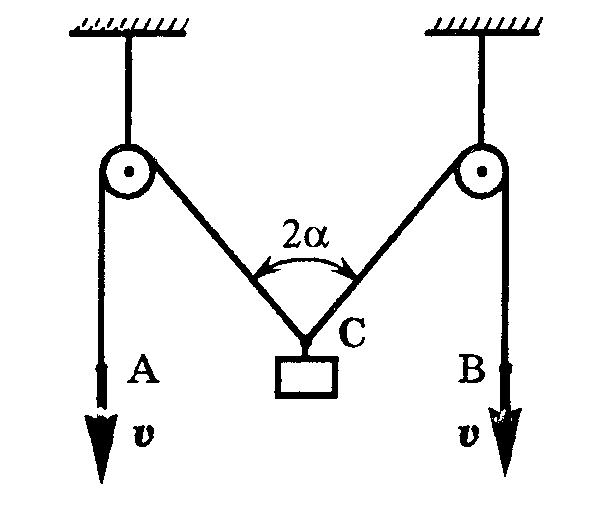
\includegraphics[width=.5\textwidth]{class3/blocks.png}
		\caption{}
		\label{day1p00}
	\end{subfigure}
	\begin{subfigure}{.4\textwidth}
		\centering
		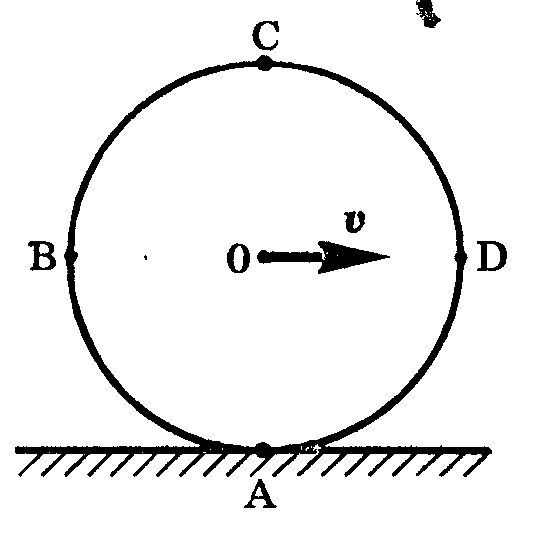
\includegraphics[width=.5\textwidth]{class3/round.png}
		\caption{}
		\label{day1p0}
	\end{subfigure}
	\caption{}
\end{figure}
\end{problem}

\begin{problem}{7}
	Котушка з намотаною на ній ниткою лежить на горизонтальному столі і може котитися по ньому без ковзання. Внутрішній радіус котушуи рівен $r$, зовнішній - $R$. З якою швидкістю $u$ буде преміщуватись вісь котушки. якщо кінець нитки тягнути в горизонтальному напрямку зі швидкістю $v$? Випадок (б) розглянути самостійно
	\begin{figure}[h!]
		\centering
		\begin{subfigure}{.4\textwidth}
			\centering
			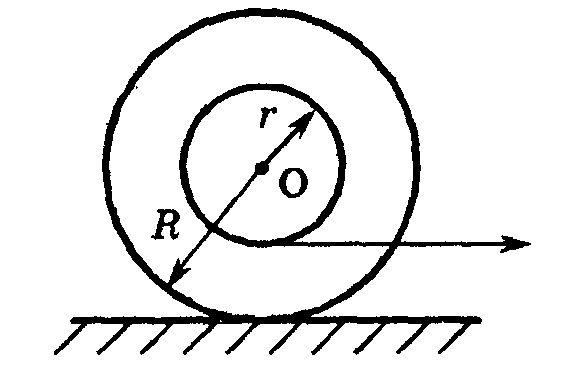
\includegraphics[width=.5\textwidth]{class3/coil_a.png}
			\caption{}
			\label{coil_a}
		\end{subfigure}
		\begin{subfigure}{.4\textwidth}
			\centering
			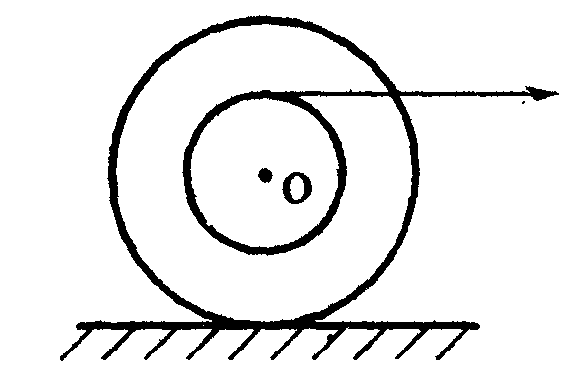
\includegraphics[width=.5\textwidth]{class3/coil_b.png}
			\caption{}
			\label{coil_b}
		\end{subfigure}
		\caption{До задачі \arabic{assigments}.\arabic{problems}}
	\end{figure}
\end{problem}


\begin{problem}{9}
	Чотири черепахи знаходяться в кутах квадрата зы стороною $a$. Черепахи починають рухатись одночасно з однаковою за модулем швидкістю $v$. При цьому перша черепаха весь час тримає курс на другу, друга -- на третю, третя -- на четверту, четверта -- на першу. 
	\begin{enumerate}
		\item Через який час $t$ черепахи зустрінуться?
		\item Дайте відповідь на задачу для трьох черепах у вершинах рівностороннього трикутника.
	\end{enumerate}
	 
\end{problem}

\textbf{Задачі для самостійного розв'язання}

\begin{problem}{4}
	Снаряд вилітає з далекобійної гармати з початковою швидкістю $v_0 = 1000~\dfrac{\text{м}}{\text{c}}$ під кутом $\alpha = 30^{\circ}$ до горизонту. Скыльки часу $t$ снаряд знаходиться в повітрі? На яку висоту $H$ снаряд піднімається? На якій відстані $L$ від гармати він впаде на землю?
\end{problem}

\begin{problem}{5}
	Під кутом $\alpha = 60^{\circ}$ до горизонту кинуто тіло з початковою швидкістю $v_0 = 20~\dfrac{\text{м}}{\text{c}}$. Через який час $t$ воно буде рухатись під кутом $\beta = 45^{\circ}$
\end{problem}

\begin{problem}{6}
	Із шланги, який лежить на землі, б'є вода під кутом $\alpha = 45^{\circ}$ до горизонту з початковою швидкістю $v_0 = 10~\dfrac{\text{м}}{\text{c}}$. Площа перерізу отвору шланги $S = 5 ~\text{см}^2$. Визначте масу m струменю, який находиться в повітрі.
\end{problem}

\begin{problem}{8}
	Кінці каната А та В (див. рис \ref{day1p00}) тягнуть з однаковою швидкістю $v$. Яку швидкість $u$ має груз в той момент, коли кут між канатами в точці його кріплення рівен $2\alpha$?
	
\end{problem}

\begin{problem}{9}
	Випадок (б) задачі 3.7 про котушку
\end{problem}